\documentclass{article}
\usepackage[utf8]{inputenc}
\usepackage{tikz}
\usepackage{circuitikz}
\usepackage{amsmath}
\usepackage{nomencl}
\usepackage{hyperref}
\usepackage{commath,amsmath}
\usepackage{pdflscape}
\usepackage{graphicx}
\graphicspath{ {../../Figures/} }
\usetikzlibrary{positioning,patterns,calc,quotes,angles}

\title{System Dynamics \\ Ball on a Beam}
\author{Ahmed Ibrahim Almohamed \\  Abdullah Albandar Alhamad }
\date{August 2023}


\begin{document}
\tableofcontents
\maketitle
\makenomenclature
\section{Abstract}

The Ball on Beam system is a classic example of control and dynamics problem that describes
the interaction of a ball place on a horizontal beam.
In this Study we will analyze the system into a mathematical model and a simulation.
We are focusing on understanding the interactions between the ball's position ,the beam's angle
and the external forces (e.g gravity).
Through the application of principles from physics and control theory,
we develop a mathematical model that describes the system's behavior.
By employing simulation techniques, we explore how the system responds to different control inputs and external disturbances.
Insights gained from this analysis contribute to a deeper understanding of the fundamental concepts of dynamics, control strategies, and stability in mechanical systems.
This research not only enhances theoretical knowledge but also provides valuable insights for designing and controlling similar systems in various practical applications.

\newpage
\printnomenclature
%%%%%%%%%%%%%%%%%%%%%%%%%%%%%%%%%%%%%%SYSTEM OVERVIEW%%%%%%%%%%%%%%%%%%%%%%%%%%%%%%%%%%%%%%%%%%%%%%%%%%%%%%%%%%%
\newpage
\section{System description}
The system comprises a ball placed on a beam that is tilted at an angle $\theta$.
The beam possesses a length $l$ and is capable of rotating around a defined pivot point.
The position of the ball on the beam is denoted by $p$, where $x = 0$ corresponds to the left end of the beam,
and $p = l$ corresponds to the right end.
The beam connects to a motor via a gear mechanism, where the distance from the motor's rotor to the gear arm is represented as $d$. The gear arrangement enables the motor to apply a torque $\tau$ to the beam, inducing its rotation about the pivot point.
Additionally, the system involves the parameter $\phi$, which signifies the gear angle.
This angle $\phi$ characterizes the orientation of the gear linked to the motor. As the motor rotates,
the gear angle $\phi$ changes, influencing the torque exerted on the beam and consequently impacting its position and tilt angle $\theta$.
The motion of the ball and the rotation of the beam are intricately linked through factors such as the motor's torque,
the gear angle $\phi$, and the distance $d$ from the rotor to the gear arm.
The system's dynamic behavior is governed by these interrelated variables,
leading to diverse motion patterns and equilibrium conditions for the ball on the tilted beam.
The comprehension and analysis of this system entail investigating the relationships among variables $l$, $x$, $d$, $\theta$, and $\phi$, as well as considering the influence of external forces like gravity and potential control inputs.
Utilizing mathematical models and principles from mechanics enables the characterization and prediction of the system's behavior across various scenarios.
% Symbols
\nomenclature{$l$}{Length of the beam}
\nomenclature{$p$}{Position of the ball on the beam}
\nomenclature{$d$}{Distance from the motor's rotor to the gear arm}
\nomenclature{$\phi$}{Gear angle}
\nomenclature{$\theta$}{Tilt angle of the beam}
\nomenclature{$r$}{Ball's radius}
\nomenclature{$\tau$}{External torque applied to the beam}
\begin{figure}[h]
	\centering
	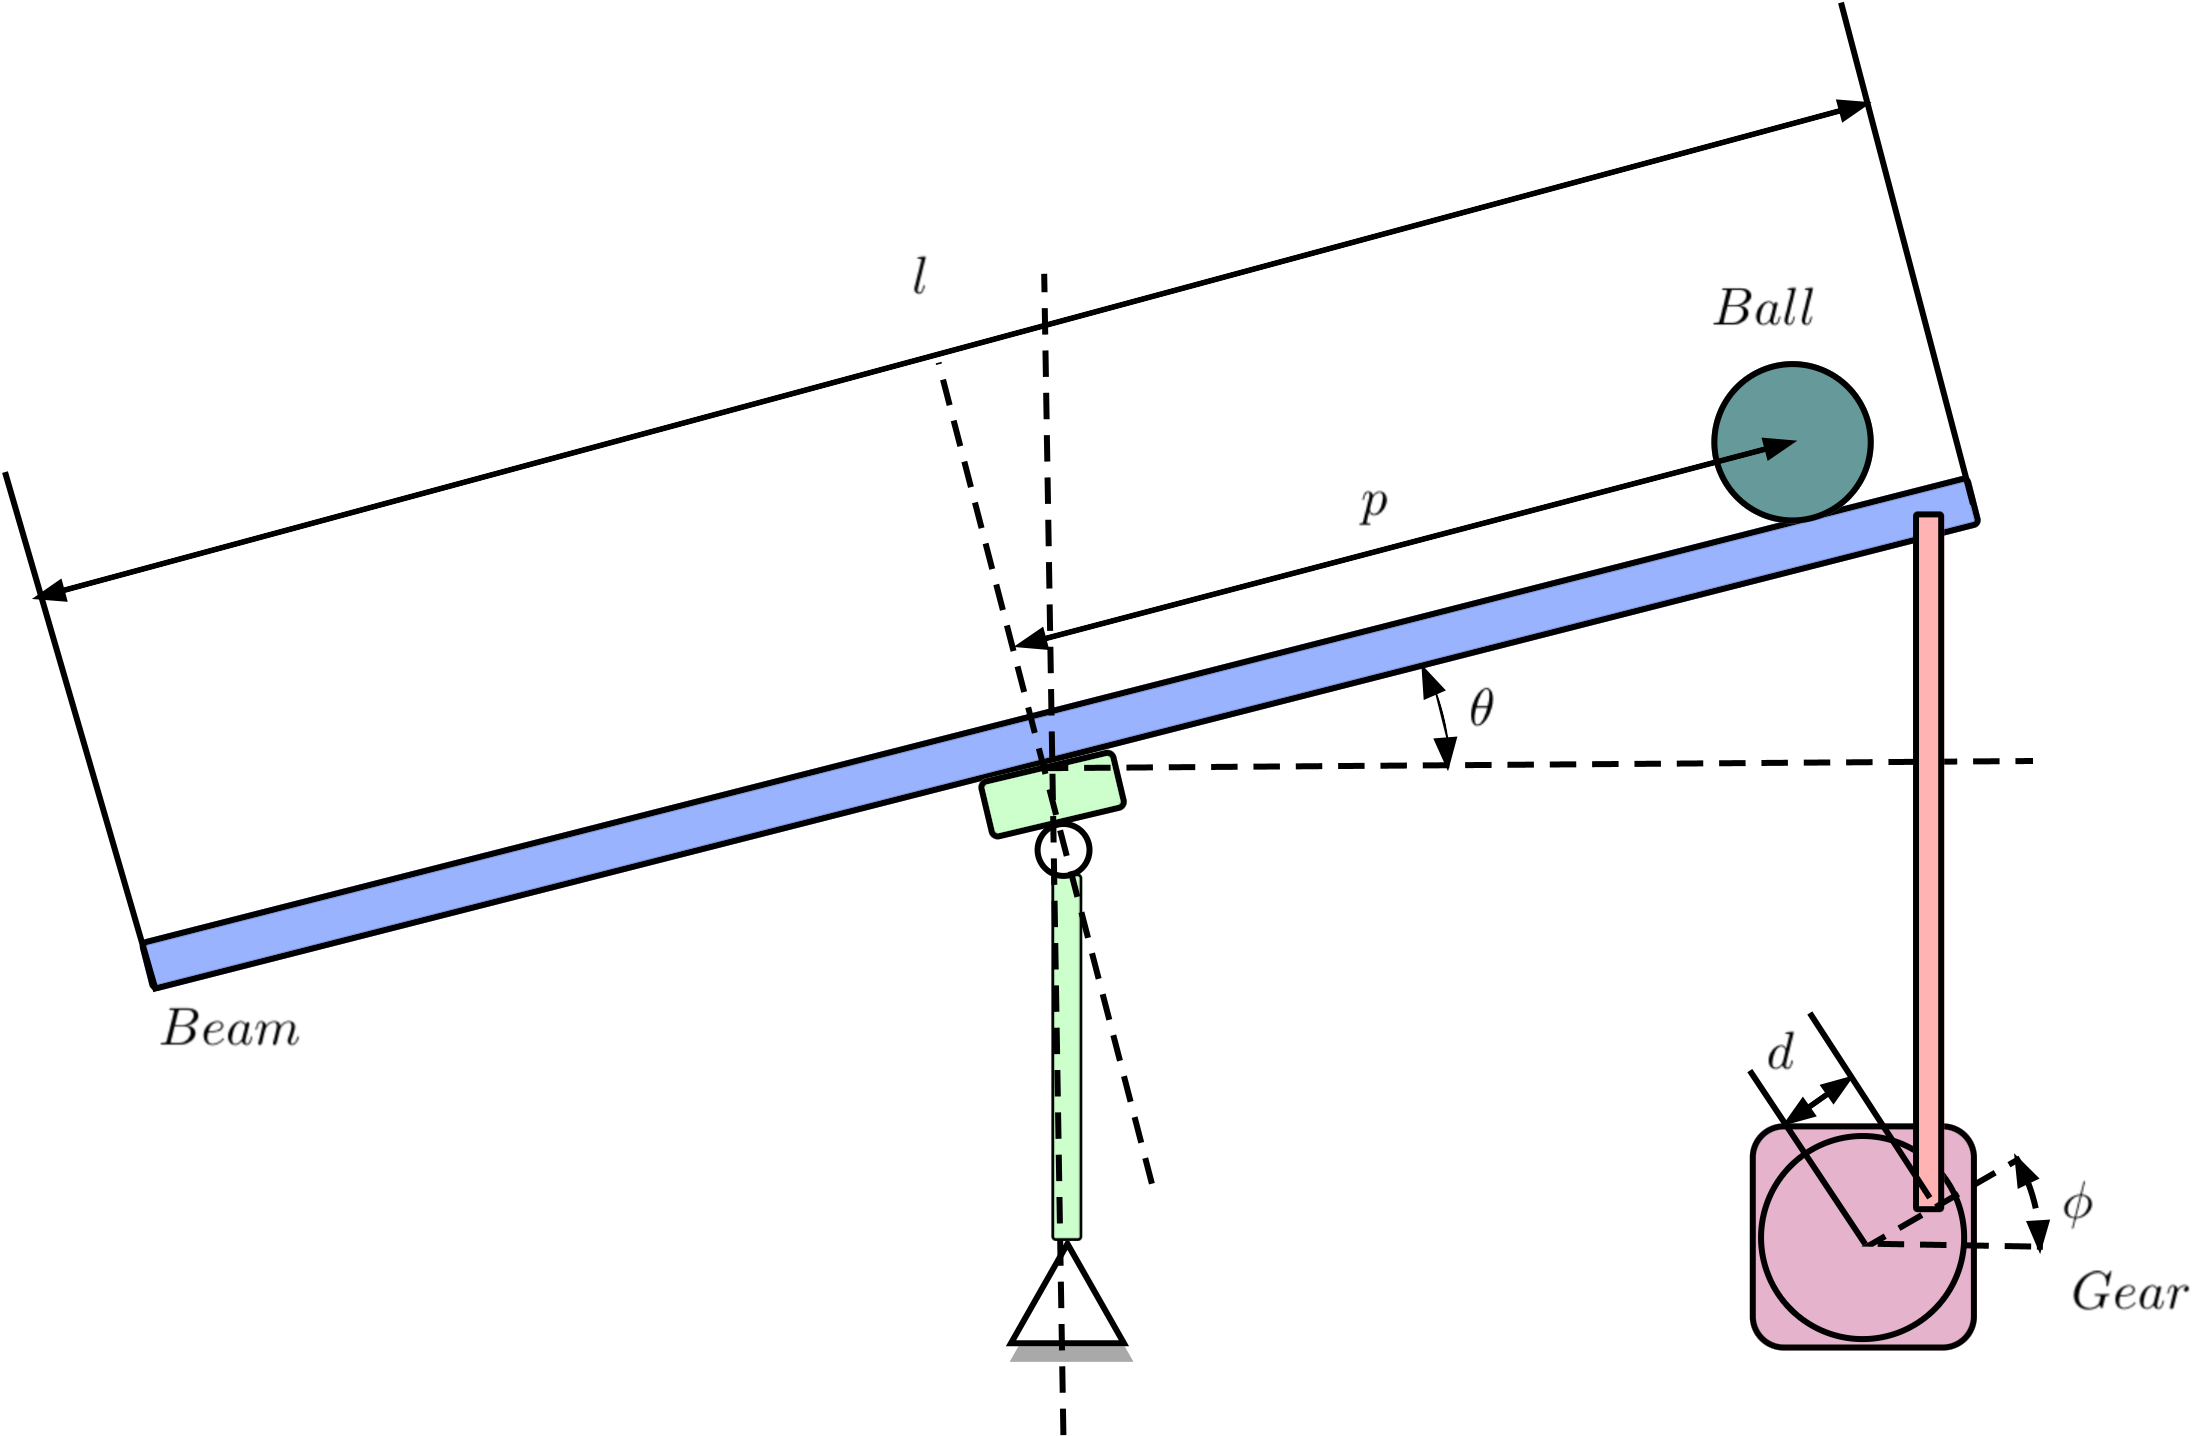
\includegraphics[height =7.5cm,width =10cm]{System_Overview}
	\caption{System Overview}
\end{figure}
%%%%%%%%%%%%%%%%%%%%%%%%%%%%%%%%%%% System geometry %%%%%%%%%%%%%%%%%%%%%%%%%%%%%
\newpage
\section{System Geometry}

\subsection{Ball's translational position and velocity}
In oder to get the system's variable right , we need to analyze the system geometry correctly.
In the \figref{SystemGeometry} we can see that the ball's center is positioned according to the distance $p$ and angle $\theta$.
But in order to find the ball's position in Cartesian , we need to transform the ball's position in terms of $x(p,\theta)$ and $y(p,\theta)$.
This will help us later when we need to change some variables from and to polar coordinates.
That we can achieve with calculating the distance from the center of rotation to the center of the ball. 

\begin{figure}[h]
	\centering
	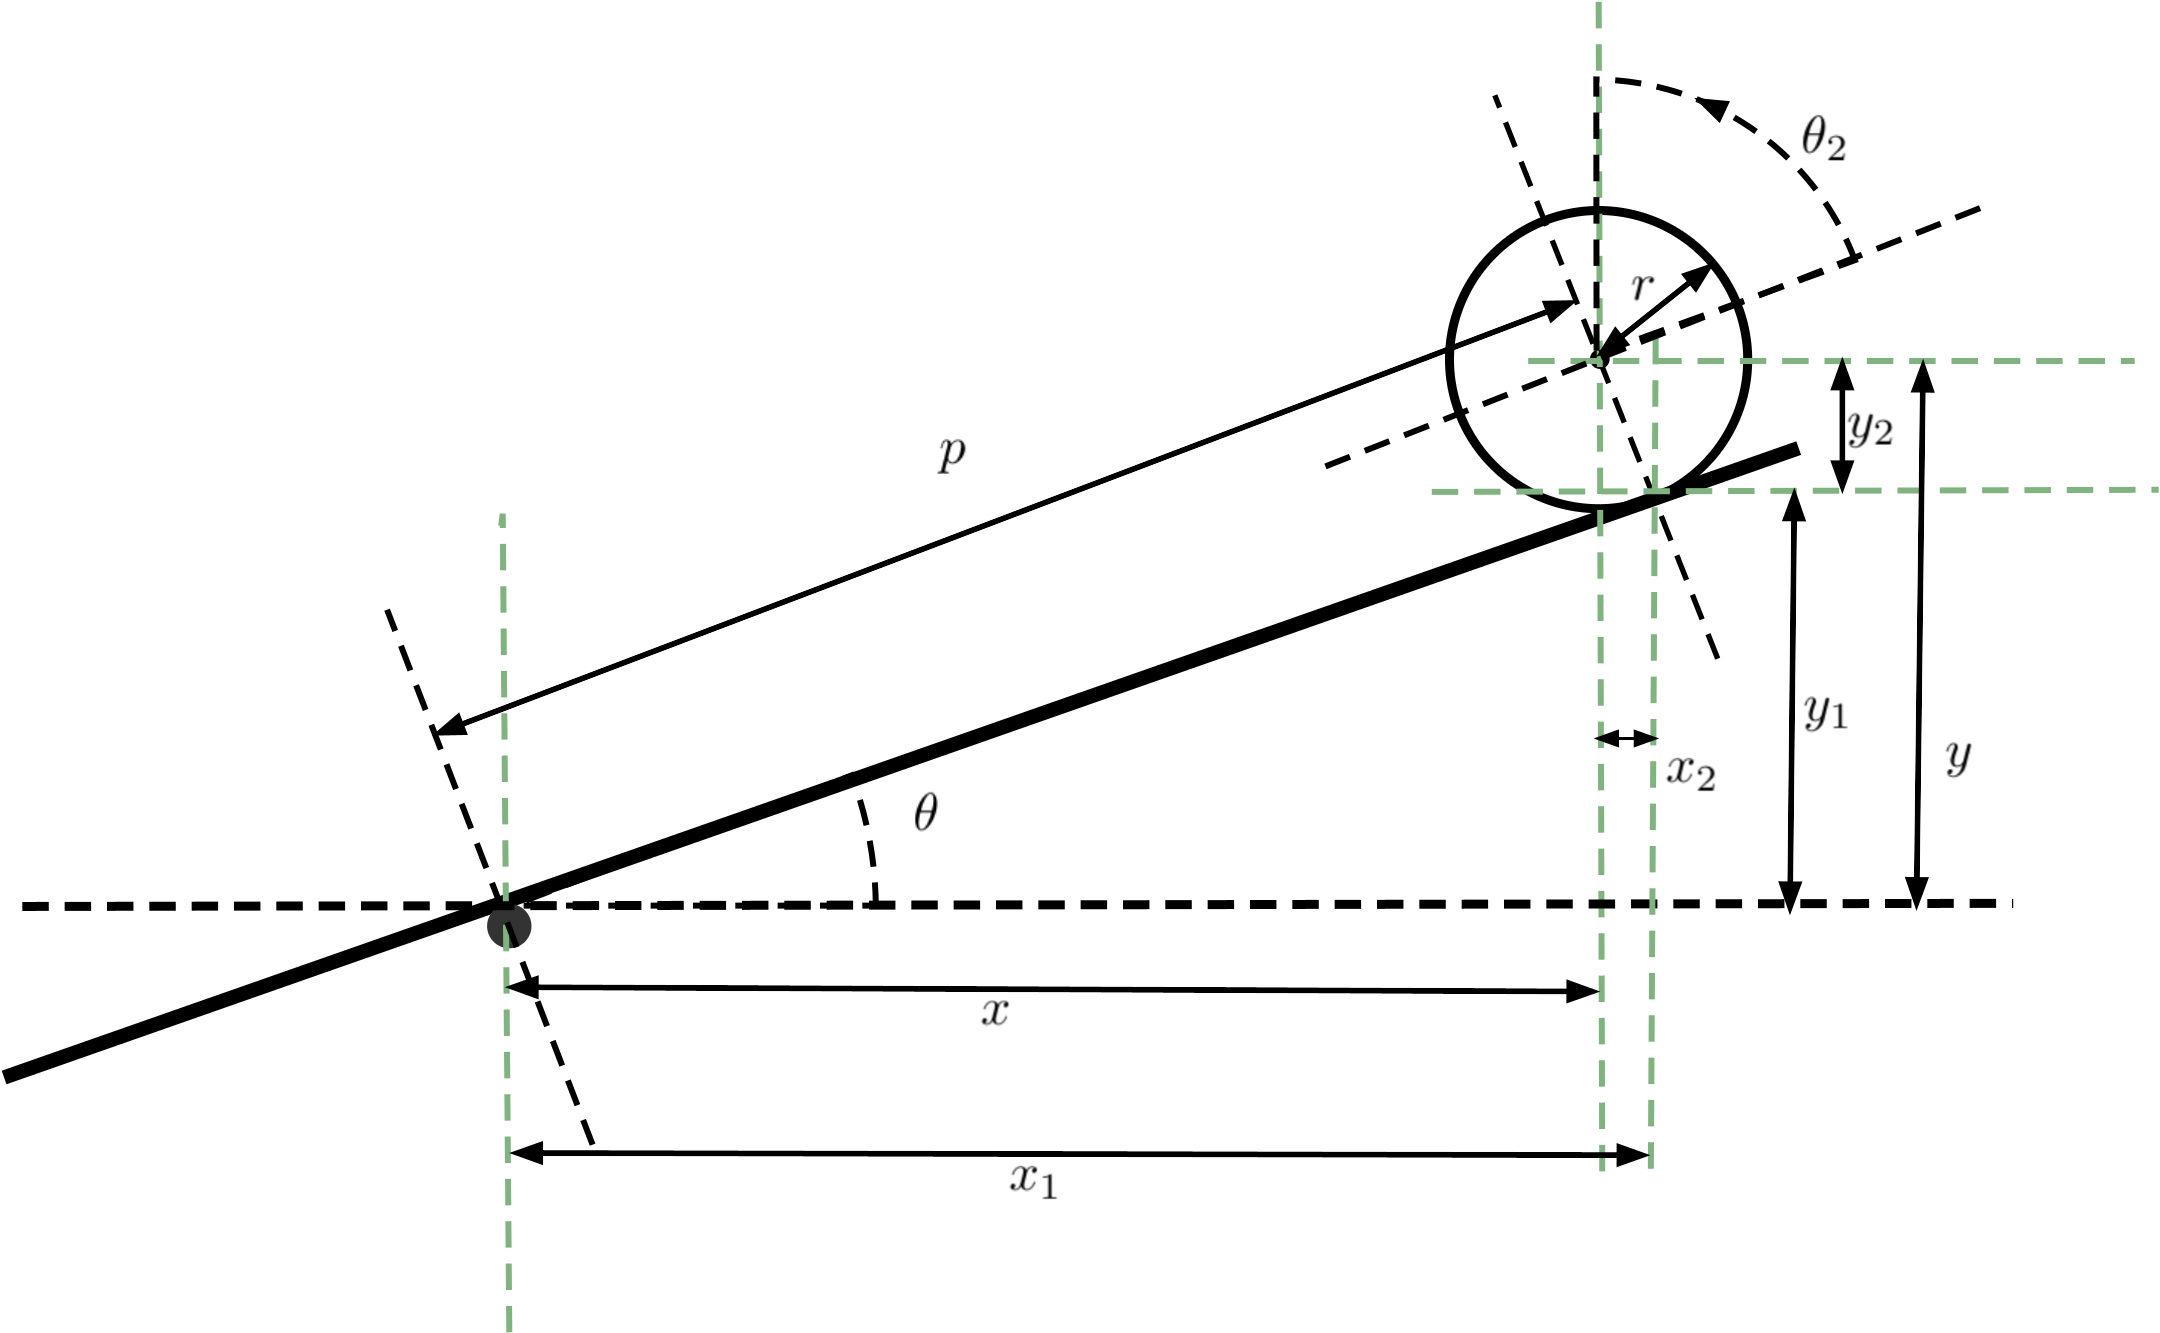
\includegraphics[height =7.5cm,width =10cm]{System_Geo}
	\caption{System Geometry}\label{SystemGeometry}
\end{figure}
\newpage
First we will consider the following while observing the \figref{SystemGeometry}:
\begin{equation}
	\begin{split}
		x = x_1 - x_2 \\
		y = y_1 + y_2 
	\end{split}
\end{equation}
Now using some trigonometry with the triangles in \figref{SystemGeometry_Triangles} we can get the following:
\begin{equation}
	\begin{split}
		x_1 = p.\cos{\theta} \\
		x_2 = r.\sin{\theta} \\
		y_1 = p.\sin{\theta} \\
		y_2 = r.\cos{\theta} 
	\end{split}
\end{equation}

\begin{figure}[h]
	\centering
	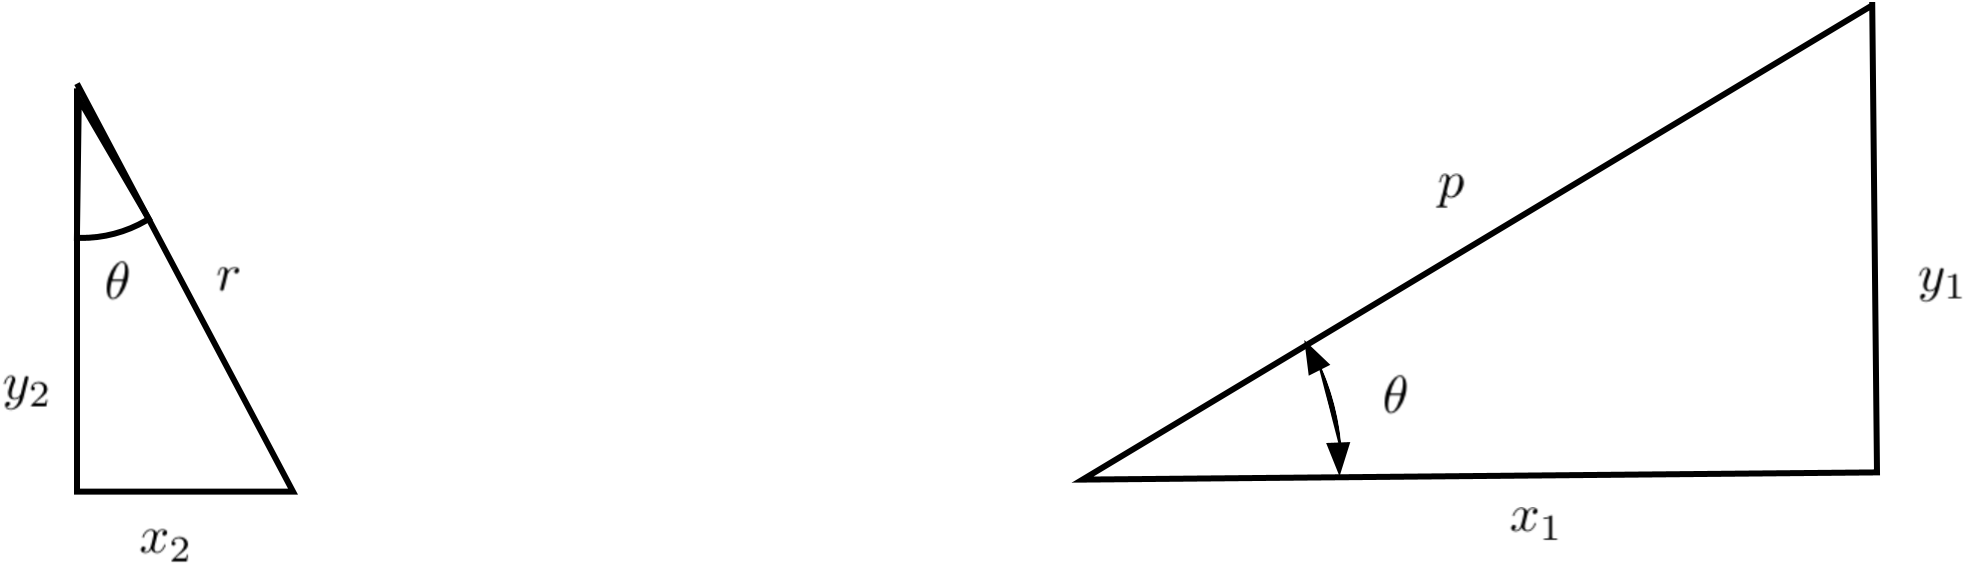
\includegraphics[height =4cm,width =8cm]{Triangles_System_Geo}
	\caption{Position Triangles}\label{SystemGeometry_Triangles}
\end{figure}
Lastly we substitute the values from (2) in (1):
\begin{equation}
	\begin{split}
		x = p.\cos{\theta} - r.\sin{\theta}\\
		y = p.\sin{\theta} + r.\cos{\theta}
	\end{split}
\end{equation}
It is also would be helpful , to calculate the velocity of the ball by taking the derivative of the position in respect to time.

\begin{equation}
	\begin{split}
		\dot{x}  = \dot{p}.\cos{\theta}-p.\theta'.\sin{\theta} - r.\theta'.\sin{\theta} \\
		\dot{y}  = \dot{p}.\sin{\theta}+ p.\theta'\cos{\theta} - r.\theta'.\sin{\theta} 
	\end{split}
\end{equation}
\newpage
\subsection{Ball's rotational position and velocity}
Now we need to find a relationship between the ball's angular values and the system variables $p$ and $\theta$.
By looking at the \figref{Angles_System_Geo} , we can tell that before tilting the system , the coordinates are normal and vertical.
After tilting the system and before the ball starts to roll , the coordinates are tilted by the amount of $\theta$,and the the ball starts to roll down, where 
a displacement of the angle is created $\alpha$,which is called the angular position of the ball.
This creates a new angle called (total displacement of the ball after tilting)$\sigma$ which is simply the sum of the two angles , and it's also equal to the position over the radius.

\begin{figure}[h]
	\centering
	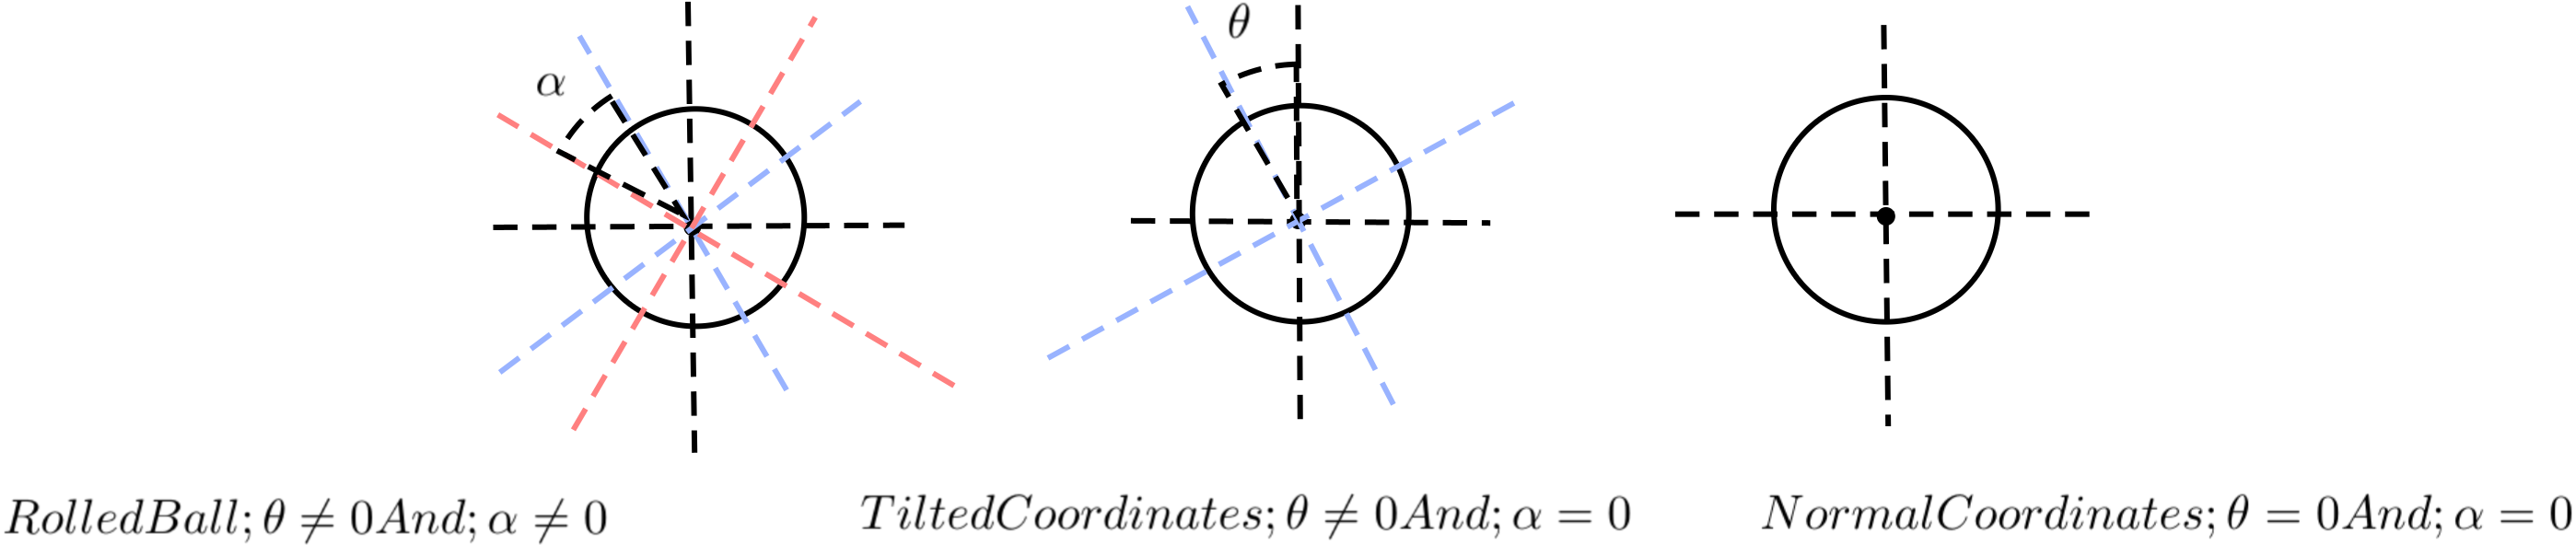
\includegraphics[height = 4cm,width =12cm]{Angles_System_Geo}
	\caption{Angular position}\label{Angles_System_Geo}
\end{figure}
Now to calculate $\alpha$:
\begin{equation}
	\begin{split}
		\sigma = \alpha + \theta \\
		\alpha = \theta - \sigma \\
		\alpha = \theta - \dfrac{p}{r}		
	\end{split}
\end{equation}
Now simply by taking the derivative of that we can calculate the angular velocity:
\begin{equation}
	\begin{split}
		\omega = \dot{\alpha} = \dot{\theta} - \dfrac{\dot{p}}{r}
	\end{split}
\end{equation}
\newpage
\subsection{Beam Geometry}

%%%%%%%%%%%%%%%%%%%%%%%%%%%%%%%%%%%%%%MATH MODEL%%%%%%%%%%%%%%%%%%%%%%%%%%%%%%%%%%%%%%%%%%%%
\newpage
\section{Mathematical model}
\noindent Using the Lagrange equation on this model we can drive the equation of motion of the system.
In order to get the Lagrange equation we need first to find both the kinetic and potential energy of the system.
Firstly we will take a look at the Ball Energy both kinetic and potential.
The Lagrange equation describes ,that the the difference between the two energies of a certain variable as a Lagrangian $L$.
The Lagrangian equation :

\begin{equation}\label{Lagrangian}
	\begin{split}
		L = E_{\text{kinetic}} - E_{\text{potential}}
	\end{split}
\end{equation}
%%%%%%%%%%%%%%%%%%%%%%%%%%%%%%%%%%%%%%%% BALL ENERGY %%%%%%%%%%%%%%%%%%%%%%%%%%%%%%%%%%%%%%%%%%
\subsection{Ball Energy}

Starting with the kinetic Energy of the Ball,it will be the summation of the translational kinetic energy and rotation energy.

\begin{equation}
	\begin{split}
		E_{\text{kineticBall}} = E_{\text{trans}} + E_{\text{rot}}
	\end{split}
\end{equation}
The translational energy is relative to the velocity of the ball,while the rotational energy is relative to the angular velocity.
The translational is then :
\begin{equation}
	\begin{split}
		E_{\text{trans}} = \frac{1}{2}.m_{\text{ball}}.v^2
	\end{split}	
\end{equation}
And the rotational energy is :
\begin{equation}
	\begin{split}
		E_{\text{rot}} = \frac{1}{2}.I_{\text{ball}}.\omega^2
	\end{split}
\end{equation}
Therefore :
\begin{equation}\label{kineticBall}
	\begin{split}
		E_{\text{kineticBall}} =\frac{1}{2}.m_{\text{ball}}.v^2 + \frac{1}{2}.I_{\text{ball}}.\omega^2
	\end{split}
\end{equation}
Now we need to calculate the ball's potential energy, 
But because of the tilted beam we can describe the potential energy with :
\begin{equation}
	\begin{split}\label{potential}
		E_{\text{potential}} = m_{\text{ball}}.g.p.\sin{\theta}
	\end{split}
\end{equation}

% Symbols :
\nomenclature{$m_{\text{ball}}$}{Mass of the ball}
\nomenclature{$\omega$}{angular velocity of the ball}
\nomenclature{$I_{\text{ball}}$}{Moment of inertia of the ball}
\nomenclature{$h$}{Height of the ball}

\newpage
\subsection{Beam Energy}
\noindent In this section we will try to describe both the kinetic and potential energy of the Beam.
Starting with the kinetic energy of the Beam ,in this case the kinetic energy comes from the rotation around a fix point in the
middle.
\begin{equation}\label{kineticBeam}
	\begin{split}
		E_{\text{kineticBeam}} = \frac{1}{2}.I_{\text{Beam}}.\omega_{\text{Beam}}^2
	\end{split}	
\end{equation}
\noindent The beam is fixed at a vertical height and is rotating around a pivot point 
in the middle, the potential energy of the beam itself can often be ignored.
The potential energy of the beam is typically negligible in comparison to other energy terms
involved in the system,
especially if the vertical height remains constant.
The potential energy of the beam arises due to its tilt angle and vertical height, 
but if the height is fixed and the tilt angle doesn't significantly affect 
the beam's position relative to the fixed height, 
the potential energy term for the beam can often be omitted from the Lagrangian.
Therefore:
\begin{equation}
	\begin{split}
		E_{\text{potBeam}} = 0
	\end{split}
\end{equation}

% Symbols
\nomenclature{$I_{\text{Beam}}$}{Moment of inertia of the Beam}
\nomenclature{$v$}{Ball's velocity on the beam}
\nomenclature{$\omega_{\text{Beam}}$}{Beam's angular velocity}
%%%%%%%%%%%%%%%%%%%%%%%%%%%%%%%%%Lagrangian Dynamics%%%%%%%%%%%%%%%%%
\subsection{Lagrangian Dynamics}
Until this point we are using the term $p$ to describe the distance of the ball on the beam.
$p$ is the polar description of the position ,which we can change into Cartesian coordinates with:

\begin{equation}
	\begin{split}
		y = p.\sin{\theta}\\
		x = p.\cos{\theta}
	\end{split}
\end{equation}
This is why the potential energy is given in terms of $p$ and $\theta$ but in realty it is in terms of $y$.
The same is applies to the velocity $v$ which is the ball's velocity on the beam in realty its a two direction on vertical and one horizontal.
That means we can describe the velocity term $v^2$ in terms of $p$ and $\theta$
\begin{equation}\label{velocity}
	\begin{split}
		v^2 = x'^2 + y'^2 
	\end{split}
\end{equation}
Where :
\begin{equation}
	\begin{split}
		x' = p.'\cos{\theta} - p.\theta'.\sin{\theta}\\
		x'^2 = p'^2.\cos^2{\theta} - 2.p.p'\theta'.\cos{\theta}.\sin{\theta}+ p^2.\theta'^2.\sin^2{\theta}
	\end{split}
\end{equation}
And :
\begin{equation}
	\begin{split}
		y'= p'.\sin{\theta}+p.\theta'.\cos{\theta} \\
		y'^2 = p'^2.\sin^2{\theta}+ 2p.p'\theta'.\cos{\theta}.\sin{\theta}+p^2.\theta'^2.\cos^2{\theta}
	\end{split}
\end{equation}
Now we substitute back to \ref{velocity}:
\begin{equation}
	\begin{split}
		v'^2 = p' + p^2.\theta'^2
	\end{split}
\end{equation}
On the other hand we can also substitute the term $\omega$ into coordinates terms $p$ and the ball radius $r$:
\begin{equation}
	\begin{split}
		\omega = \frac{p}{r}
	\end{split}
\end{equation}
We can plug this back to \ref{kineticBall} so we can describe the kinetic energy of the ball in term of $p$ and $\theta$:
\begin{equation}
	\begin{aligned}
		E_{\text{kineticBall}} = \frac{1}{2}.m_{\text{ball}}.(p' + p^2.\theta'^2) + \frac{1}{2}.I_{\text{ball}}.\frac{p^2}{r^2}\\
		= \frac{1}{2}.(\frac{I_{\text{ball}}}{r^2}+m_{\text{ball}}).p'^2 + \frac{1}{2} m_{\text{ball}}.p^2.\theta'^2
	\end{aligned}
\end{equation}
After defining the main kinetic and potential energy of the system we can set the 
equations into the Lagrangian \ref{Lagrangian} .
\begin{multline}
		L = \frac{1}{2}.(\frac{I_{\text{ball}}}{r^2}+m_{\text{ball}}).p'^2 + \frac{1}{2} m_{\text{ball}}.p^2.\theta'^2 +\\
		\frac{1}{2}.I_{\text{Beam}}.\omega_{\text{Beam}}^2- m_{\text{ball}}.g.p.\sin{\theta}
\end{multline}
We simplify it to :
\begin{equation}
	\begin{split}
		L = \frac{1}{2}.(\frac{I_{\text{ball}}}{r^2}+m_{\text{Beam}}).p'^2 + \frac{1}{2}(m_{\text{ball}}.p^2 + I_{\text{Beam}}).\theta'^2 - m_{\text{ball}}.g.p.\sin{\theta} 
	\end{split}
\end{equation}
%%%%%%%%%%%%%%%%%%%%%%%%%%% Lagrangian equations of Motion %%%%%%%%%%%%%%%%%%%%%%%%%%%

\newpage
\subsection{Lagrangian equations of Motion}
The Lagrangian equations of motion use to describe the how the system behave according to the terms of $p$ and $\theta$
Equations are :

\begin{equation}\label{LEM first}
	\begin{split}
		\od{}{t}(\pd{L}{p'}) - \pd{L}{p} = 0
	\end{split}
\end{equation}
And :
\begin{equation}\label{LEM second}
	\begin{split}
		\od{}{t}(\pd{L}{\theta'}) - \pd{L}{\theta} = \tau
	\end{split}	
\end{equation}
Now solving for \ref{LEM first}
\begin{equation}
	\begin{split}
		\pd{L}{p'} = 2.\frac{1}{2}.(\frac{I_{\text{ball}}}{r^2}+m_{\text{ball}}).p'\\
			= (\frac{I_{\text{ball}}}{r^2}+m_{\text{ball}}).p'
	\end{split}	
\end{equation}
Then :
\begin{equation}
	\begin{split}
		\od{}{t}(\pd{L}{p}) = (\frac{I_{\text{ball}}}{r^2}+m_{\text{ball}}).p''
	\end{split}
\end{equation}
And the other term :
\begin{equation}
	\begin{split}
	\pd{L}{p} = m_{\text{ball}}.p.\theta'^2 - m_{\text{ball}}.g.\sin{\theta}
	\end{split}
\end{equation}
Thus the result of the first Lagrangian equation :
\begin{equation}
	\begin{split}
		(\frac{I_{\text{ball}}}{r^2}+m_{\text{ball}}).p'' +  m_{\text{ball}}.p.\theta'^2 - m_{\text{ball}}.g.\sin{\theta} = 0
	\end{split}
\end{equation}
Next we solve the second equation \ref{LEM second}:
\begin{equation}
	\begin{split}
		\pd{L}{\theta'} = (m_{\text{ball}}.p^2 + I_{\text{Beam}}).\theta'
	\end{split}
\end{equation}
And : 
\begin{equation}
	\begin{split}
		\od{}{t}(\pd{L}{\theta'}) = (m_{\text{ball}}.p^2 + I_{\text{Beam}}).\theta'' + 2.m_{\text{ball}}.p.p'.\theta'
	\end{split}
\end{equation}
And the other term :
\begin{equation}
	\begin{split}
		\pd{L}{\theta} = -m_{\text{ball}}.g.p.\cos{\theta}
	\end{split}
\end{equation}
Thus the the result of the second Lagrangian equation:
\begin{equation}
	\begin{split}
		(m_{\text{ball}}.p^2 + I_{\text{Beam}}).\theta'' + 2.m_{\text{ball}}.p.p'.\theta' + m_{\text{ball}}.g.p.\cos{\theta} = \tau
	\end{split}
\end{equation}
These two equations describe how the external torque effects the system as an input to the system, and how the distance $p$ and the angle $\theta$ are changed accordingly.
%%%%%%%%%%%%%%%%%%%%%%%%%%%%%%%%%%%%% State Space %%%%%%%%%%%%%%%%%%%%%%%%%%
\newpage
\section{State-Space Model}
First, in order to build the State Space model of the system we need to simplify the constants terms of the system.
This will be achieved by looking into the constants of the two Lagrangian equations and mash the constants into new constants.
From the first Lagrangian equation :
\begin{equation}
	\begin{split}
		(\frac{I_{\text{ball}}}{r^2}+m_{\text{ball}}) = \alpha \\
		g.m_{\text{ball}} = \beta
	\end{split}
\end{equation}
And from the second Lagrangian equation:
\begin{equation}
	\begin{split}
		2.m_{\text{ball}} = \gamma \\
	\end{split}
\end{equation}
What we really have in this system are two differential equations of second order with two variables $p$ and $\theta$.
We can rewrite the system as four differential equations of first order.
These two system are not linear due to the quadratic and trigonometrical terms in them, which means that the system needs to linearized around equilibrium point(s).
Now we will rename the variables $p$ ,$p'$,$\theta$ and $\theta'$ into :
\begin{equation}
	\vec{x} =
	\begin{bmatrix}
		x_1 \\
		x_2 \\
		x_3 \\
		x_4 \\
	\end{bmatrix}=
	\begin{bmatrix}
		p \\
		p' \\
		\theta \\
		\theta '
	\end{bmatrix}
\end{equation}
Also the input torque will be renamed :
\begin{equation}
	\begin{split}
		\tau = u
	\end{split}
\end{equation}
Now the vector $\vec{x}$ holds all the system variables in itself and we can rewrite the Lagrangian equations with it.

\begin{equation}
	\begin{split}
		\alpha.x_2' +  m_{\text{ball}}.x_1.x_4^2 - \beta.\sin{x_3} = 0 \\
		(m_{\text{ball}}.x_1^2 + I_{\text{Beam}}).x_4' + \gamma.x_1.x_2.x_4 + \beta.x_1.\cos{x_3} = u
	\end{split}
\end{equation}
Now we will write a general form of the State Space :

\begin{equation}
	\vec{\dot{x}} =
	\begin{bmatrix}
		x_1' \\
		x_2' \\
		x_3' \\
		x_4' \\
	\end{bmatrix} =
	\begin{bmatrix}
		x_2\\
		\frac{ m_{\text{ball}}.x_1.x_4^2 - \beta.\sin{x_3}}{\alpha} \\
		x_4\\
		\frac{- \gamma.x_1.x_2.x_4 - \beta.x_1.\cos{x_3}}{(m_{\text{ball}}.x_1^2 + I_{\text{Beam}})}
	\end{bmatrix}+
	\begin{bmatrix}
		0 \\
		0\\
		0\\
		\frac{1}{(m_{\text{ball}}.x_1^2 + I_{\text{Beam}})}
	\end{bmatrix}*u
\end{equation}
Also the output of the system is a signal output which is the position of the ball at a time $t$.
Therefore:
\begin{equation}
	\begin{split}
		\vec{y} = x_1
	\end{split}
\end{equation}
%%%%%%%%%%%%%%%%%%%%%%%%%%%%%%%%%%%% Linearization of the State-Space %%%%%%%%%%%%%%%%%%%%%%%
\newpage
\subsection{Linearization of the State-Space}
In order to set the equilibrium point(s) we must be careful about the $x_1$ which represent the position (here :initial) of the ball.
Setting this initial value to 0 will cause the equations to draft to infinity ,which is not possible.
This means that we need to chose an equilibrium where all the other values except $x_1$ is set to zero, while $x_1$ is set 1.
In other word , The Ball has no initial velocity , the beam's angle is zero and has no angular velocity but the ball is positioned at 1 unit of measurement.
\begin{equation}
	\vec{x_*} =
	\begin{bmatrix}
		x_{\text{$1_*$}} \\
		x_{\text{$2_*$}} \\
		x_{\text{$3_*$}} \\
		x_{\text{$4_*$}}
	\end{bmatrix}=
	\begin{bmatrix}
		1 \\
		0 \\
		0 \\
		0 \\
	\end{bmatrix}
\end{equation}
We need also to find equilibrium point of the External torque $u$ which we will set also to zero.

\begin{equation}
	\begin{split}
		u_* = 0
	\end{split}
\end{equation}
Further to do, is to find the jacobian matrix around the equilibrium point(s) ,by doing this we will reach a linearized state-space model of the system,
which we can test ,simulate and find more about the project before we start the implementation.
Also to reach the normal form of the State-space which is :

\begin{equation}
	\begin{split}
		\vec{\dot{x}} = A*\vec{x} + B*\vec{u};\\
		\vec{y}  = C*\vec{x} + D*\vec{u}
	\end{split}
\end{equation}
The jacobian will give us the linearized matrices $\Delta A$,$\Delta B$,$\Delta C$ and $\Delta D$.
\begin{equation}
	\begin{split}
		\Delta A = \pd{\vec{\dot{x}}}{\vec{x}}\|x_*,u_*\\
		\Delta B = \pd{\vec{\dot{x}}}{\vec{u}}\|x_*,u_*\\
		\Delta C = \pd{\vec{y}}{\vec{x}}\|x_*,u_* \\
		\Delta D = \pd{\vec{y}}{\vec{u}}\|x_*,u_*
	\end{split}
\end{equation}
Now we need to find the value of these matrices.
Starting with $\Delta A$ evaluating it at $\vec{x_*}$ and $u_*$
\begin{equation}
	\Delta A =
	\begin{bmatrix}
		0 &1 &0 &0\\
		0 &0 & -\frac{\beta}{alpha} &0\\
		0 &0 &0 &1 \\
		-\frac{\beta.(m_{\text{ball}} -I_{\text{Beam}} )}{(m_{\text{ball}}+I_\text{Beam})^2} & 0 & 0 & 0
	\end{bmatrix}
\end{equation}
\newpage
Then $\Delta B$ is :

\begin{equation}
	\Delta B =
	\begin{bmatrix}
		0 \\
		0 \\
		0 \\
		\dfrac{1}{m_{\text{ball}} +I_{\text{Beam}} }
	\end{bmatrix}
\end{equation}
To Get $\Delta C $
\begin{equation}
	\Delta C =
	\begin{bmatrix}
		1 & 0 & 0 & 0
	\end{bmatrix}
\end{equation}
And when calculate $\Delta D $ ,,we found that simply it is zero ,because there is no $u$ term in the $\vec{y}$ equation.
Therefore :
\begin{equation}
	\begin{split}
		\Delta D = 0
	\end{split}
\end{equation}

\newpage
\section{Stability}

\end{document}